\section{Setup}
\begin{frame}
\frametitle{Test set-up}

\begin{enumerate}[<+->]
	\setlength\itemsep{1em}
	\item User arrival rates were modelled in 8 phases.
	\item The work flow consisted of 4 distinct sessions with various probabilities.
	\item Interspersed waiting within sessions.
	\item Specialized tests were set up to test caching and indexing.  
\end{enumerate}
\end{frame}

\begin{frame}
\frametitle{Session 1}
\begin{figure}[h]
	\centering
	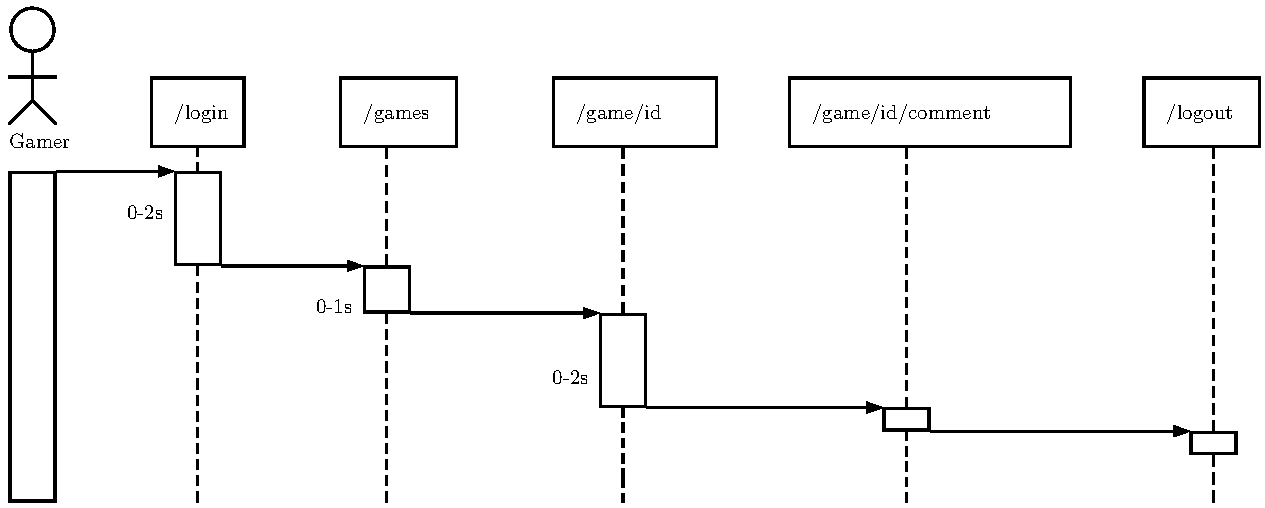
\includegraphics[width=1\textwidth, height=0.5\textheight]{images/generic-1.pdf}
	\caption{First Session}\label{fig:sqlopt}
\end{figure}
\end{frame}

\begin{frame}
\frametitle{Session 2}
\begin{figure}[h]
	\centering
	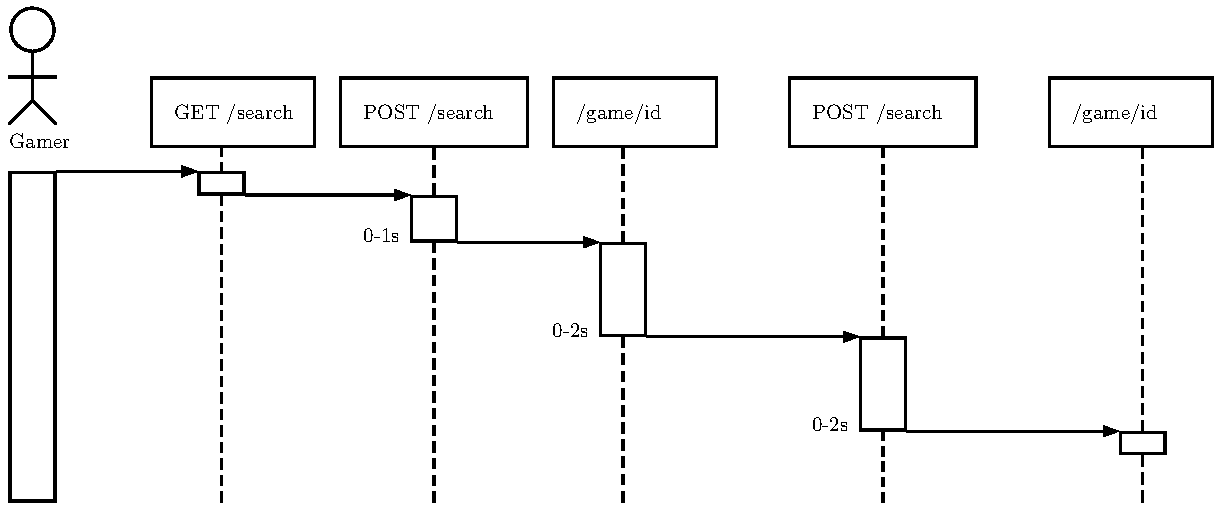
\includegraphics[width=1\textwidth, height=0.5\textheight]{images/generic-2.pdf}
	\caption{Second Session}\label{fig:sqlopt}
\end{figure}
\end{frame}

\begin{frame}
\frametitle{Session 3}
\begin{figure}[h]
	\centering
	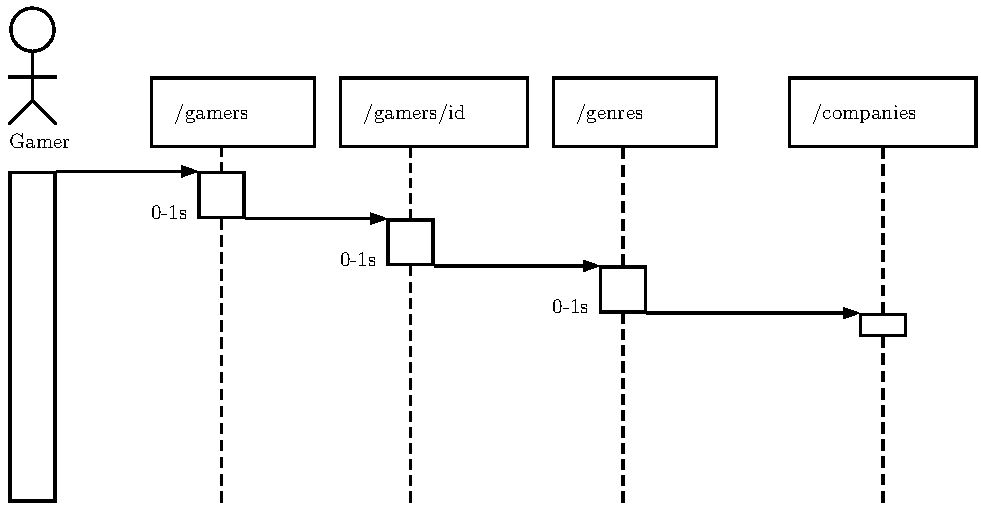
\includegraphics[width=1\textwidth, height=0.5\textheight]{images/generic-3.pdf}
	\caption{Third Session}\label{fig:sqlopt}
\end{figure}
\end{frame}

\begin{frame}
\frametitle{Session 4}
\begin{figure}[h]
	\centering
	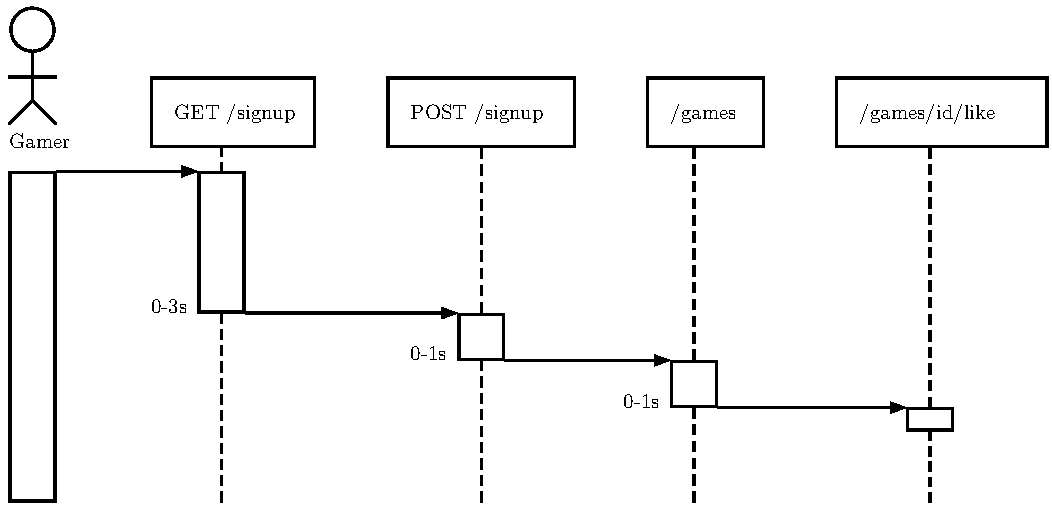
\includegraphics[width=1\textwidth, height=0.5\textheight]{images/generic-4.pdf}
	\caption{Fourth Session}\label{fig:sqlopt}
\end{figure}
\end{frame}
